\title{Multilayer Perceptron}
\label{chp:multilayer-perceptron}
\author{Lucas Costa \and Márcio Guerreiro \and Erickson Puchta \and Yara de Souza Tadano \and Thiago Antonini Alves \and  Maurício Kaster \and Hugo Valadares Siqueira}
\institute{}
\maketitle

Artificial Neural Networks (ANNs) are parallel and distributed systems inspired by higher organisms' nervous system behavior. They are based on processing units called artificial neurons, capable of calculating mathematical functions \cite{haykin}. They can learn to process information to produce the expected output\cite{Castro2006FundamentalsON}.

In general, ANNs emulate how the nervous system performs a specific function or task, having a natural tendency to store knowledge based on experiences and allow its use. This capability, linked to the modulation of the value of connections between neurons, gives ANNs the character of general tools for solving different problems. Thus, they are often applied in tasks such as pattern classification, data mining, regression/approximation of functions, and information processing, being useful in several areas of knowledge \cite{haykin}.

The conception of ANNs begins with understanding the operation of the artificial neuron. The concept from which the study started to reach complex structures establishes the investigation field of computational neuroscience or neurocomputing. This field has gained popularity thanks to its efficient ways of learning \cite{Russell2009}.

In detail, this chapter will discuss the multilayer perceptron (MLP), the best-known ANN architecture.  Previously, it was essential to introduce the artificial neuron concept, the primary processing structure of an MLP.

%%%%%%%%%%%%%%%%%%%%%%%%%%%%%%%%%%%%%%%%%%%%%%
\section{Artificial Neuron}
\label{sec:neuronio}

The biological neuron inspires the artificial neuron. Neural impulses are received through dendrites and processed in the cell body. Depending on the result of the integration of the received signals, if they are higher than a critical threshold, the neuron may or may not produce a new impulse (action potential), which will, in turn, be transmitted to other neurons connected to its axon terminals \cite{Castro2006FundamentalsON}. The axon union with dendrites is called a synapse, which works as a valve controlling the flow of information (impulses) between neurons. The synapse is variable, hence, with the ability to adapt and learn.

Figure \ref{fig:neuronio} shows the generic artificial neuron scheme used in ANNs. This device receives a set of $\textbf{u} = [ u_1 , u_2 ,..., u_i]$ inputs from other neurons or the network input, processes this information, and responds with a $y$ signal. This response, a transformation of the received inputs, is propagated to other neurons.

\begin{figure}[h!]
	\caption{Scheme of an artificial neuron built with $u_i$ inputs and $y$ outputs.}
	\vspace{0.2cm}
	\begin{center}
		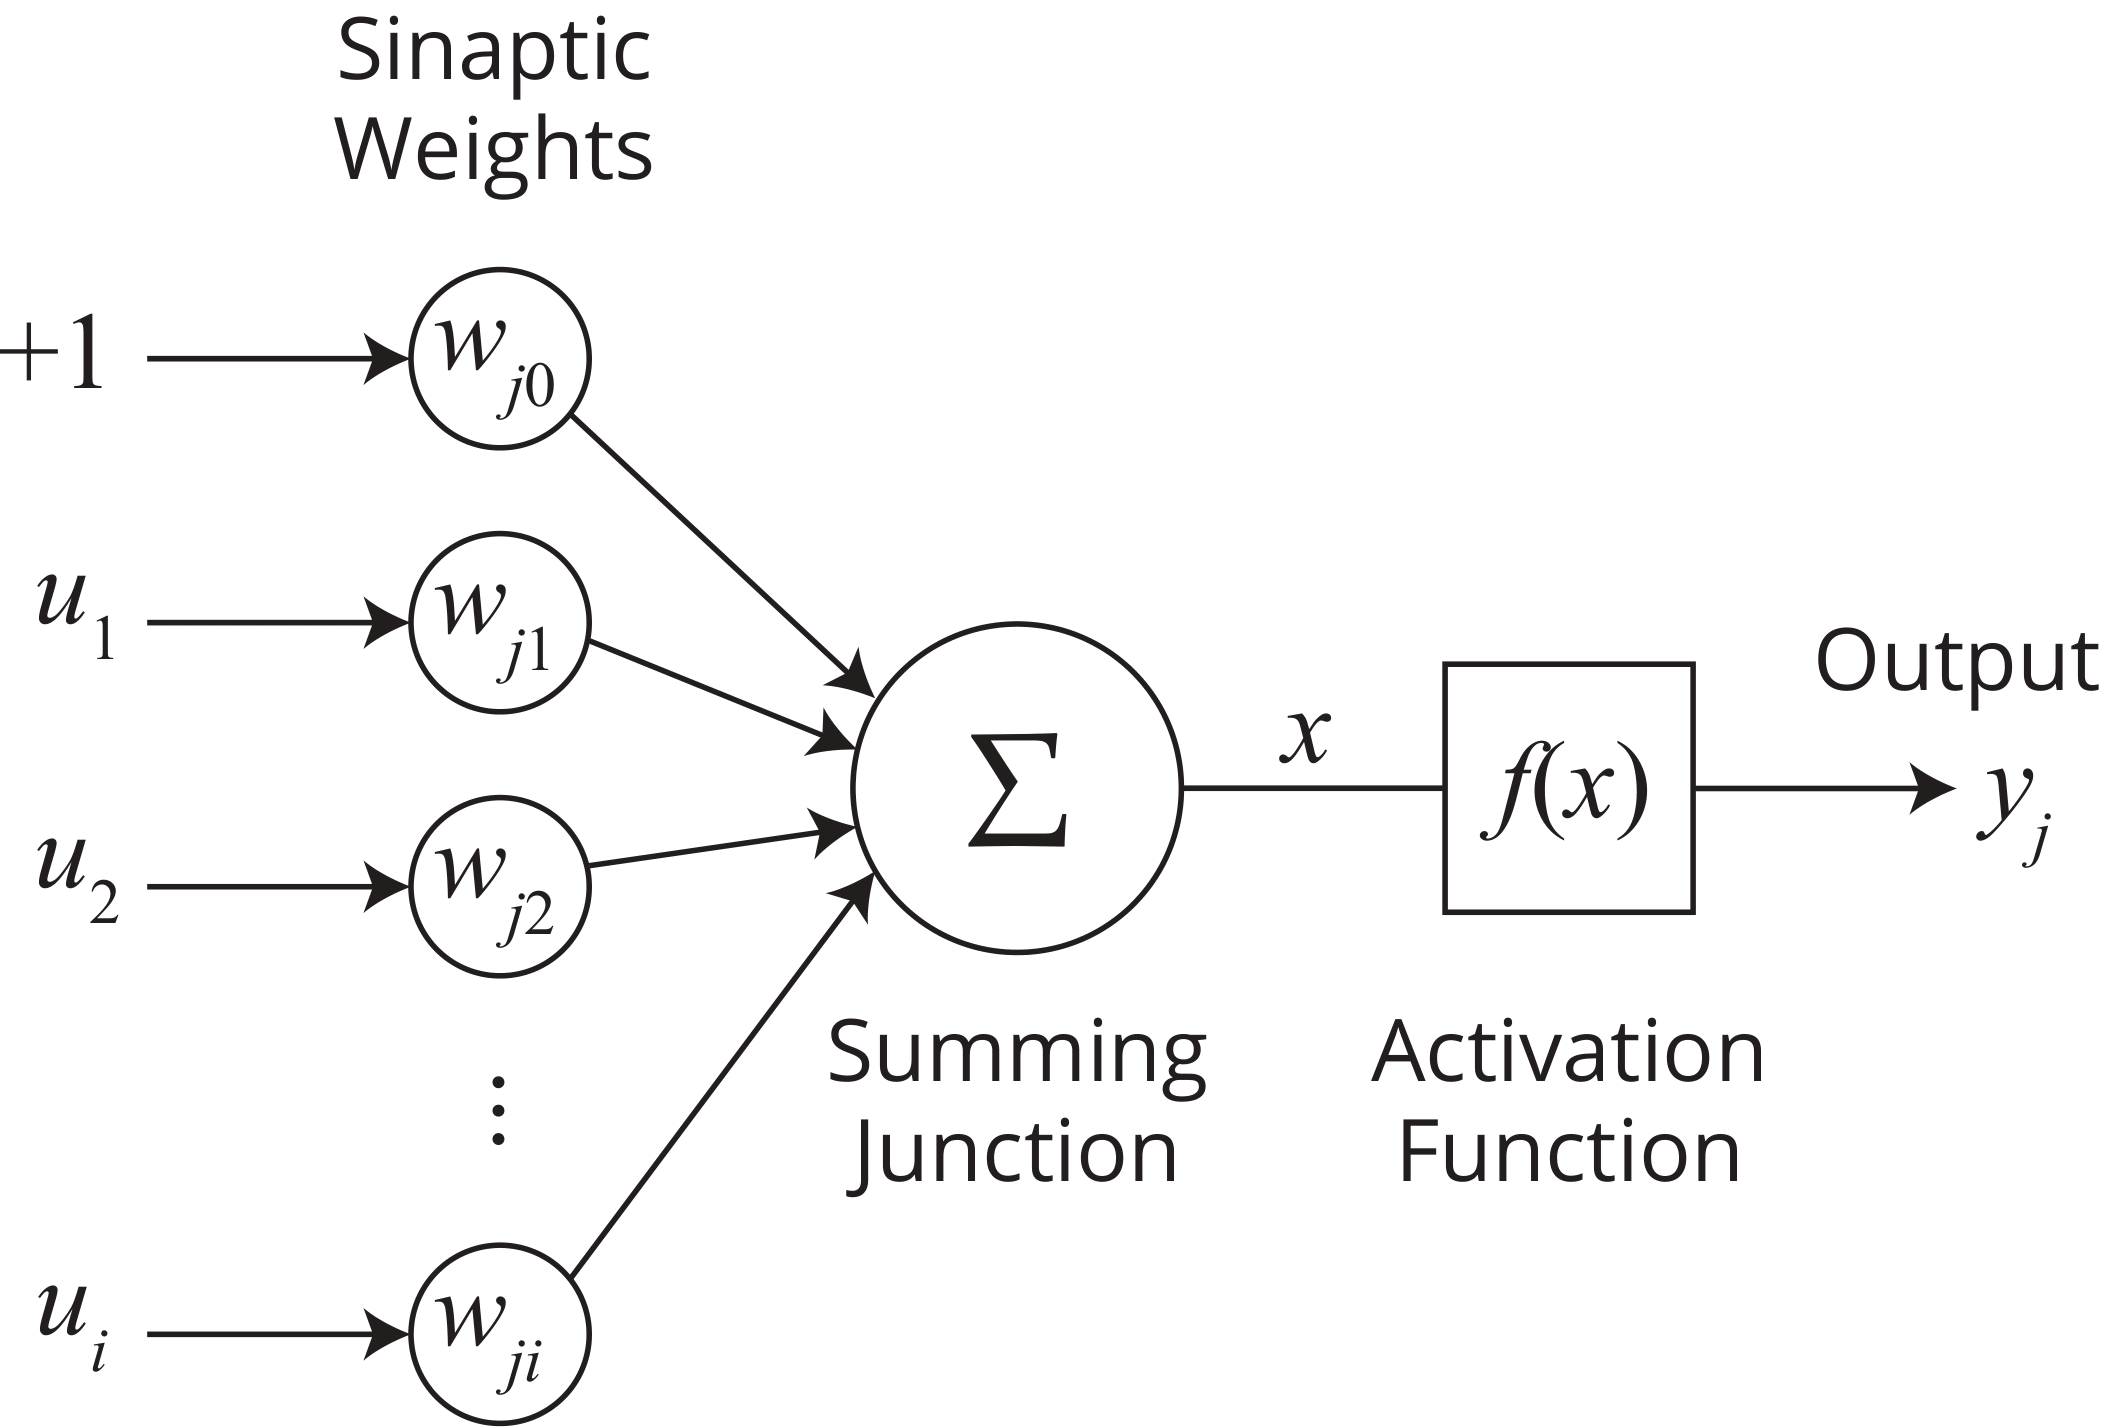
\includegraphics[width=0.8\textwidth]{"Part 3 - Learning Systems/Supervised Learning/Multilayer Perceptron/neuronioArtificial.png"}
	\end{center}
	\label{fig:neuronio}
\end{figure}

This figure shows that the input signals $u_i , i=1, 2,..., I$ and a fixed value bias signal $+1$ are weighted by the weights $w_{ji}$ in each neuron $j$. The activation $x$ (induced local field) is reached with these terms, which goes through the activation function $f(\cdot)$, generating the output $y_j$. In general, the activation function $f(\cdot)$ is nonlinear. The mathematical representation of this model is given by Equation \ref{eq:neuronio}, where the index $i=0$ represents the bias:
\begin{equation}
    \label{eq:neuronio}
    y_j = f \left( \sum_{i=0}^I w_{ji} u_i  \right).
\end{equation}

Next chapter will describe more information about the activation functions.

%%%%%%%%%%%%%%%%%%%%%%%%%%%%%%%%%%%%%%%%%%%%%%%
\subsection{Activation Functions}
\label{ssec:ativacao}

An activation function $f(\cdot)$ defines the output of a given neuron, respecting the integration (activation) value $x$. Several functions have already been used or developed, which allow the production of results with actual values, not only binary outputs, as in the case of Perceptron \cite{haykin}.

The linear activation function is widely used in output layer neurons. It's a simple function that can be described by equation \ref{eq:funcaoAtivacaoLinear}: \begin{equation}
	\label{eq:funcaoAtivacaoLinear}
	f(x) = \alpha x,
\end{equation}
where $\alpha$ is a real number.

Another standard function is the signal, also known as \textit{Heaviside} \cite{haykin}, which can respond in a binary $\{0, 1\}$ or bipolar $\{-1, 1\}$ way, the first being the one used in the McCulloch and Pitts neuron \cite{McCulloch1990}, as shown in Equation \ref{eq:funcaoAtivacaoMCP}:
\begin{equation}
	\label{eq:funcaoAtivacaoMCP}
	y = f(x) = \left\{\begin{matrix}
		0, & x < 0    \\
		1, & x \geq 0 \: .
	\end{matrix}\right.
\end{equation}

A group of functions most commonly used in the hidden layers of an MLP is the sigmoid functions \cite{haykin, Castro2006FundamentalsON}. Its graph has the peculiar shape of an ``S". It presents a balance between linear and nonlinear behavior, obtained from several functions, such as the logistic function and the hyperbolic tangent \cite{Jeffrey2008}. The logistic function can be defined as Equation \ref{eq:funcaoAtivacaoLogistica}:
\begin{equation}
	\label{eq:funcaoAtivacaoLogistica}
	f(x) = \frac{1}{1 + e^{-x}}\:.
\end{equation}

Therefore, the hyperbolic tangent is defined by Equation \ref{eq:funcaoAtivacaotanh}:
\begin{equation}
\label{eq:funcaoAtivacaotanh}
	f(x) = \frac{e^x - e^{-x}}{e^x + e^{-x}}\:.
\end{equation}

The wide use of S-Shaped functions is also due to some essential features \cite{Menon1996}:

\begin{itemize}
    \item This function is continuous and differentiable at all points, allowing adjustment with derivative-based algorithms such as gradient;
    \item It has output saturation, which ends up preventing the output signal of each neuron from diverging;
    \item It is possible to use them to create different mappings since these functions have an almost linear character in the region around the origin. At the same time, close to saturation, they are strongly nonlinear.
\end{itemize}

Recently, with the advancement of ANNs studies and, more specifically, \textit{deep learning} methods, new activation functions were developed to solve vanishing gradients or flat surfaces \cite{Fahlman1988}.

One new activation function, the Rectified Linear Unit or ReLU \cite{Maas2013}, can be expressed by Equation \ref{eq:relu}.
\begin{equation}
	\label{eq:relu}
	f(x) = \left\{\begin{matrix}
		x, & x > 0    \\
		0, & x \leq 0 \:.
	\end{matrix}\right.
\end{equation}

\noindent
If $x$ is greater than zero, the output will equal the input.

The ReLU function is similar to the linear activation function (Equation \ref{eq:funcaoAtivacaoLinear}) for values greater than zero. %, com exceção da presença de um número real $\alpha$. 

Another newly developed function is the Exponential Linear Unit or ELU \cite{Clevert2016}. Its definition is expressed by Equation \ref{eq:relu}:

\begin{equation}
	\label{eq:elu}
	f(x) = \left\{\begin{matrix}
		x,               & x > 0    \\
		\alpha(e^x - 1), & x \leq 0 \:,
	\end{matrix}\right.
\end{equation}

The definition for $x$ lower than zero allows solutions with negative values.

%%%%%%%%%%%%%%%%%%%%%%%%%%%%%%%%%%%%%%%%%%%%%%%%%%%%%%%%%%
\section{MLP Architecture}
\label{sec:mlp}

One of the best-known ANN architectures is the multilayer perceptron (MLP), which structurally generalizes the Rosenblatt perceptron \cite{Rosenblatt1958}. As demonstrated by \cite{Cybenko1989}, this ANN has universal approximation capability: an MLP can approximate any continuous, bounded, differentiable, nonlinear function with defined inputs in a compact space with arbitrary precision. It is possible by the additive composition of base functions, which, for MLP, are ridge functions. However, this theorem does not specify the amount of artificial neurons required, nor does it define any method for adjusting the value of the weights so that the optimal configuration of the network is guaranteed.

A layer is the arrangement of parallel neurons, which receive all the signals from the previous inputs but do not communicate with each other, and only send the response forward, known as a \textit{feedforward} structure. Several layers of neurons can be chained together, with the initial layer being the input; the final, outgoing; and the inner layers are called intermediate layers or hidden layers. The hidden layers are responsible for mapping the input signal in a nonlinear way in another space, according to the demand of the problem. Figure \ref{fig:mlp} shows one of the possibilities for building an MLP, with one hidden layer and one output.

\begin{figure}[h!]
    \centering
    \caption{Example of building an MLP.}
    \vspace{0.2cm}
    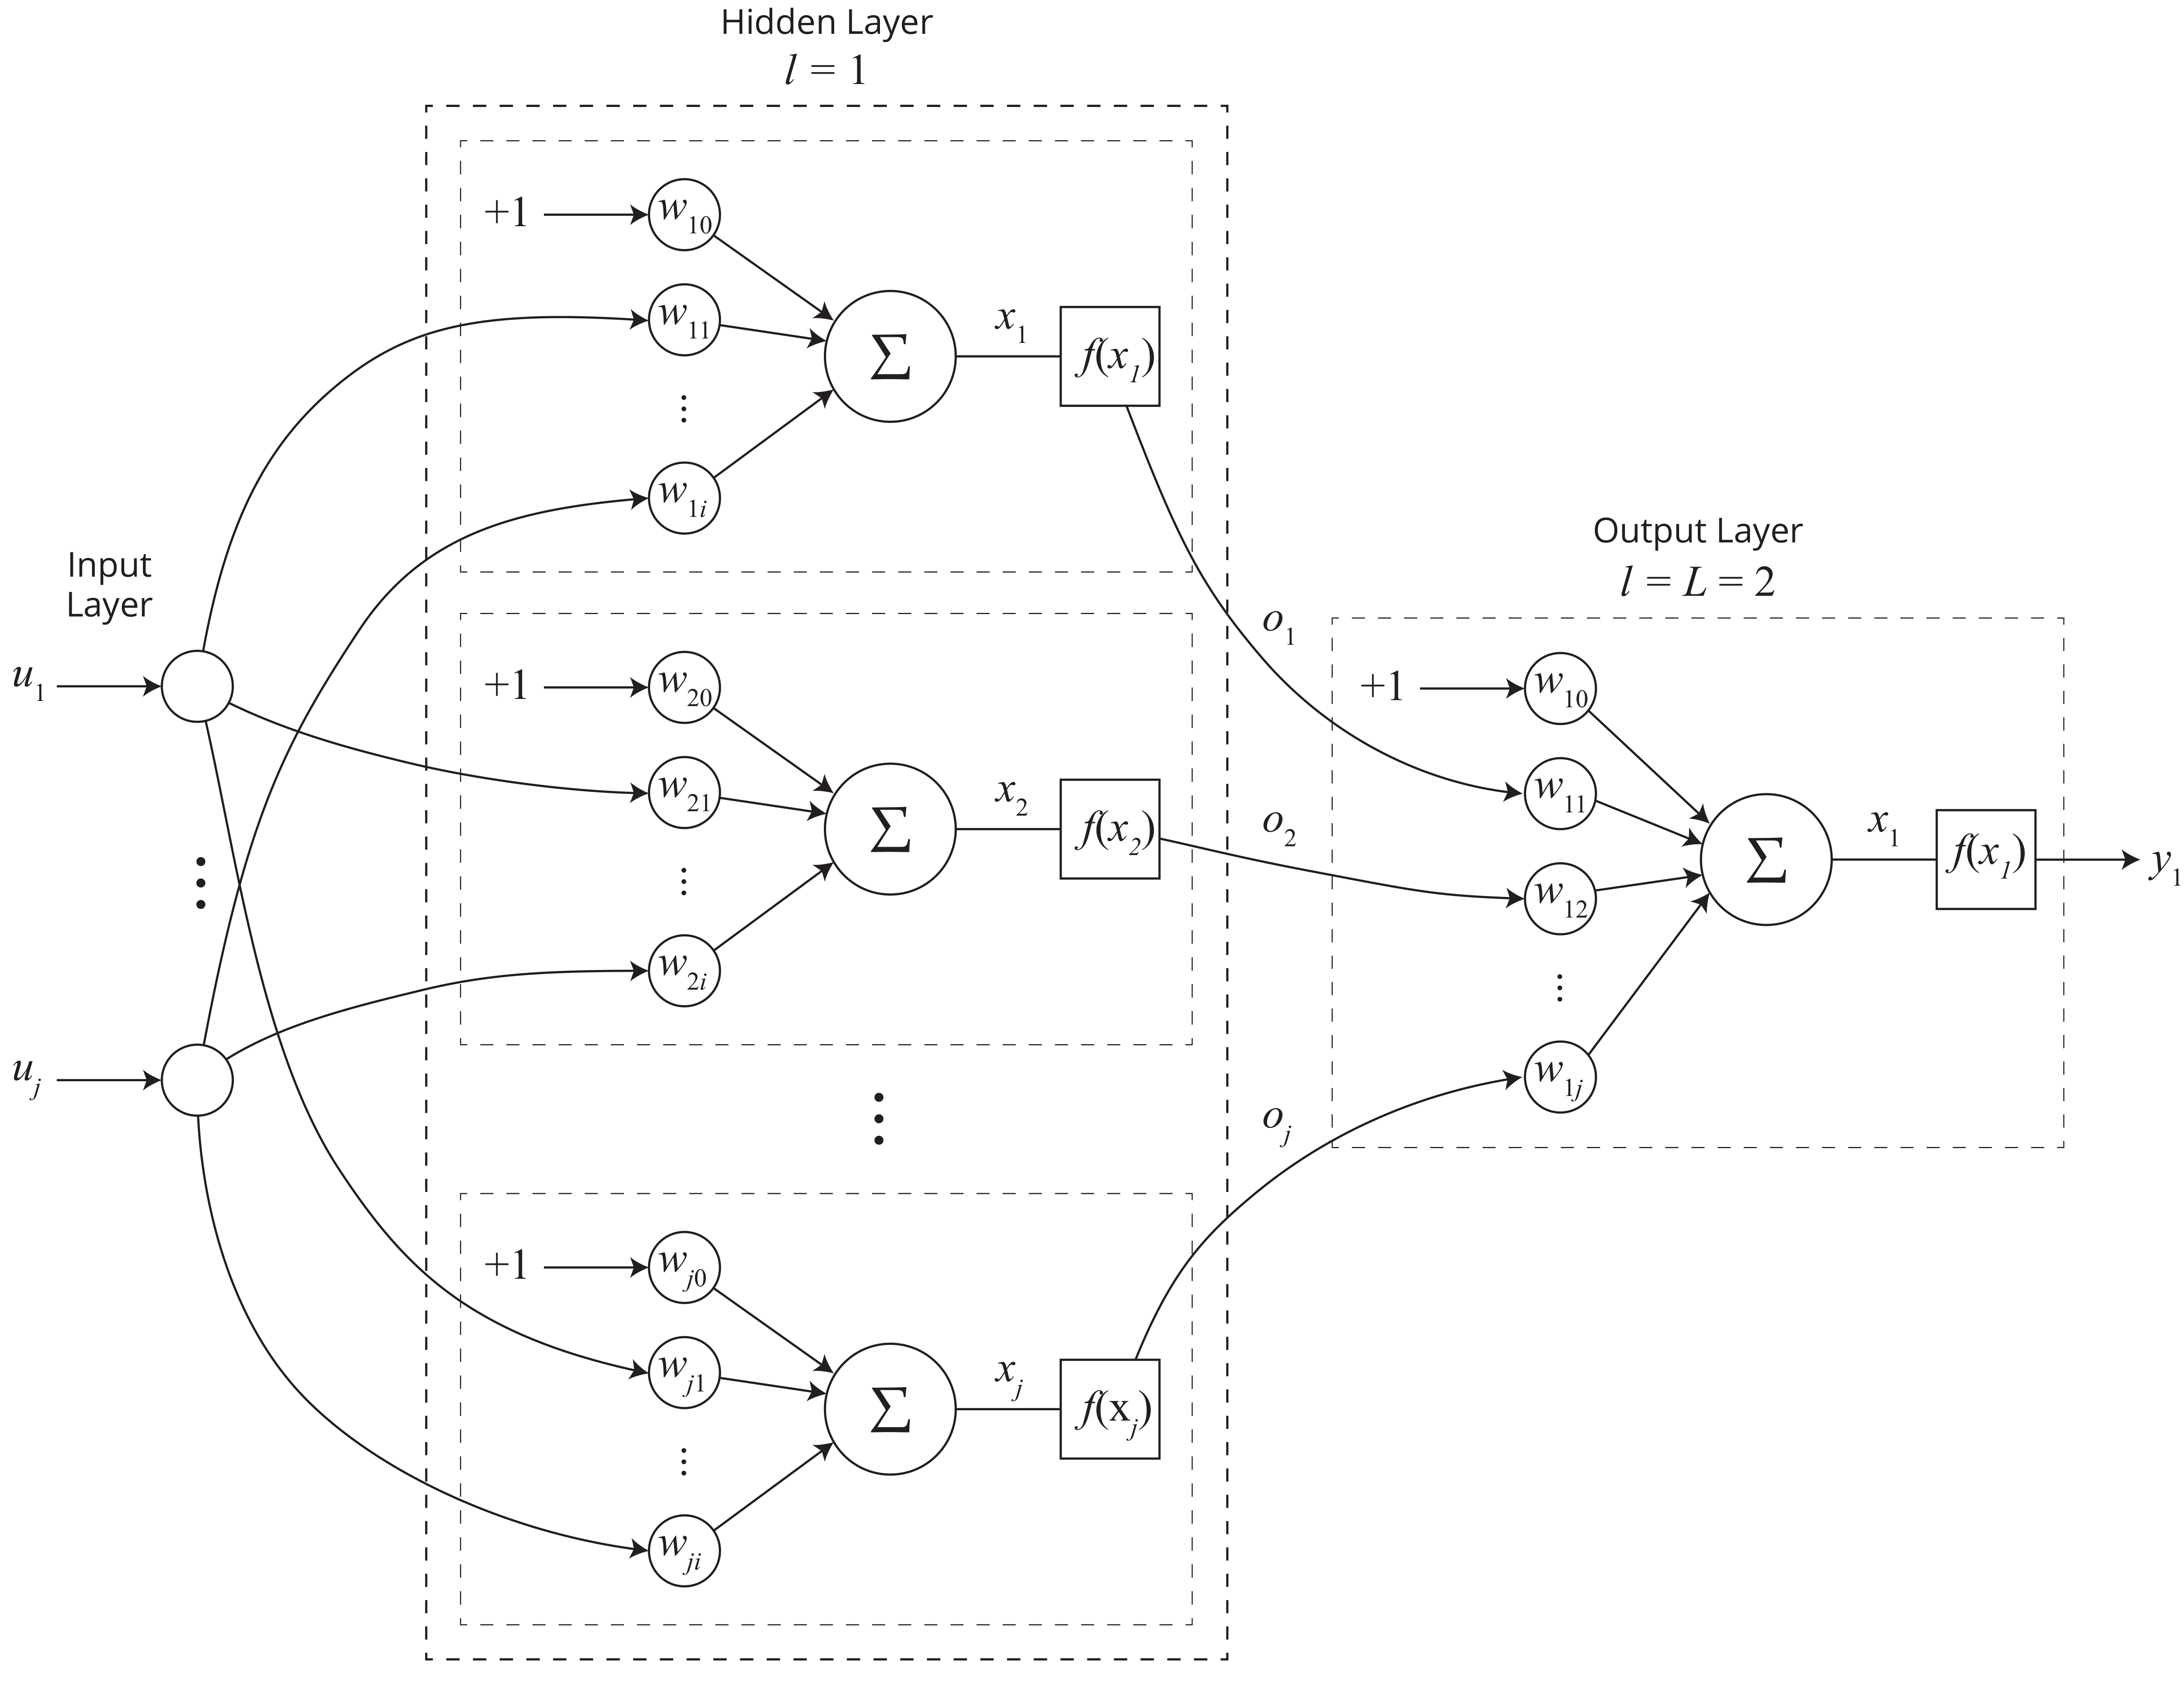
\includegraphics[width=1\textwidth]{"Part 3 - Learning Systems/Supervised Learning/Multilayer Perceptron/MLP.png"}
    \label{fig:mlp}
\end{figure}

MLPs can contain several layers in between, but it is common to employ only one or two in practical applications \cite{haykin}.

%%%%%%%%%%%%%%%%%%%%%%%%%%%%%%%%%%%%%%%%%%%%%%%%%%%%%%%%%%%%
\section{Training}
\label{ssec:treino}

There are several training algorithms aimed at adjusting the weights of an MLP. This chapter will focus on the traditional descending gradient method with the famous backpropagation \cite{rumelhart1986learning}.

The training process of an MLP is typically supervised and consists of two steps: forward and backward. In the first stage, the network weights do not change; they are fixed, and the input data is propagated to the network output. Then, an error signal is produced, comparing the outcome of the network with the desired response. After, the gradient vector of the error function is calculated. Finally, the descending gradient method is applied from the last to the first layer, making subsequent adjustments in the weights between connections \cite{haykin}. In section \ref{ssec:Pseudocodigo}, this procedure is presented in a mathematical format.

The most used error measure for this task is the mean squared error (MSE), where training algorithms will minimize concerning weights. This procedure is nothing more than an unconstrained nonlinear optimization problem. It can be treated by any unconstrained nonlinear optimization method of 1st or 2nd orders, such as the gradient and Levenberg-Marquardt methods. Note that such a premise is not based on original biological inspiration.

Backpropagation makes use of an iterative optimizing algorithm to reduce the calculated error. Since the default algorithm used with backpropagation is the descending gradient, the goal is to take repeated steps in the opposite direction of the function's gradient at the current point. These iterations, called cycles or epochs, are executed until some stopping criterion is reached \cite{Castro2006FundamentalsON}.

There are different learning methods to handle the adjustment of network weights based on the descending gradient \cite{haykin, Bengio2012}:

\begin{itemize}
	\item Batch learning: weight adjustments occur after all samples are presented to the network, at the end of each epoch during the training;
	\item Online learning: at each sample, the weights are updated, turning the search for a solution in the multidimensional weight space happen stochastically since the examples are presented in random order;
	\item Mini-batch learning: an intermediate process between learning in Batch learning and Online learning, performing updates after computing fixed batch sizes.
\end{itemize}

%%%%%%%%%%%%%%%%%%%%%%%%%%%%%%%%%%%%%%%%%%%%%%%%%%%%%%%%%%%%
\subsection{Backpropagation}
\label{ssec:Pseudocodigo}

The first phase in applying backpropagation is the propagation of the input signal passing through the hidden layers until reaching the output layer (forward). For this to happen, the network has its weights initialized randomly and then follows the presentation of training data. If there is some previous knowledge about the mapping process being worked on, it is possible to initialize the weights with pre-fixed values. Below, we followed the definitions of Simon Haykin \cite{haykin}.

Consider as training data ($\mathbf{u}(n), \mathbf{d}(n)$) for iteration $n$, where $\mathbf{u}(n)$ is the input vector applied to the ANN input layer, and $\mathbf{d} (n)$ is the desired response vector. The input signal propagation is done by calculating the $x_j^{(l)}(n)$ induced local fields for neuron $j$ in layer $l$ (Equation \ref{eq:backprop1}):

\begin{equation}
\label{eq:backprop1}
    x_j^{(l)}(n) = \sum_i w_{ji}^{(l)}(n) y_i^{(l-1)}(n),
\end{equation}
for $y_i^{(l-1)}(n)$ equal to the output signal of the neuron $j$ of the previous layer $l-1$, and $w_{ji}^{(l)}(n)$ being the weight of the neuron $j$ in layer $l$ that is powered by neuron $i$ in layer $l-1$.

When $i=0$, or $y_0^{(l-1)}(n) = +1$, this is the sign of the bias applied to the neuron $j$ of the layer $l$. The output of neuron $j$ from layer $l$ can be defined by Equation \ref{eq:backprop2}:

\begin{equation}
\label{eq:backprop2}
    y_j^{(l)} = f_j (x_j (n) ),
\end{equation}

If the neuron $j$ is in the first hidden layer ($l = 1$), then Equation \ref{eq:backprop3} is used:

\begin{equation}
    \label{eq:backprop3}
    y_j^{(0)} = u_j (n),
\end{equation}
where $u_j(n)$ is the $j$th element of the input vector $\mathbf{u}(n)$. 

However, if the neuron $j$ is in the output layer ($l = L$) for $L$ equals the total number of layers of the network, then Equation \ref{eq:backprop4} is used:

\begin{equation}
    \label{eq:backprop4}
    y_j^{(L)} = o_j (n).
\end{equation}

Afterward, the error for each neuron in the output layer is calculated. It starts the second phase of the backpropagation (backward): the propagation of the error and adjustment of the weights. This adjustment can be seen as an optimization problem that minimizes a cost function based on an approximation error metric. The next step is to compute the error signal according to Equation \ref{eq:backprop5}:
\begin{equation}
    \label{eq:backprop5}
    e_j (n) = d_j(n) - o_j (n),
\end{equation}
with $d_j (n)$ being the $j$th element of the desired response vector $\mathbf{d}(n)$.

Afterward, the local gradients $\delta$ of the network are calculated. The local gradient of the output layer $L$ is obtained by Equation \ref{eq:backprop6}:
\begin{equation}
    \label{eq:backprop6}
    \delta_j^{(L)} (n) = e_j^{(L)}(n) {f}'_j (x_j^{(L)}(n)),
\end{equation}
and those of the other layers are following Equation \ref{eq:backprop7}:
\begin{equation}
    \label{eq:backprop7}
    \delta_j^{(l)} (n) = {f}'_j (x_j^{(l)}(n)) \sum_k \delta_k^{(l+1)} (n) w_{kj}^{(l+1)}(n),
\end{equation}
for the $k$-th neuron directly behind the $j$-th neuron, where ${f}'_j(\cdot)$ is the derivative of the objective function concerning the argument.

Finally, the adjustment of the weights of the layer $l$ takes place according to the generalized delta rule of Equation \ref{eq:backprop8}:
\begin{equation}
    \label{eq:backprop8}
    w_{ji}^{(l)} (n+1) = w_{ji}^{(l)}(n) + \eta \delta_j^{(l)}(n) y_i^{(l-1)} (n).
\end{equation}

One way to improve the weight adjustment process and avoid instabilities is to modify Equation \ref{eq:backprop8} by adding a term from \textit{momentum}, changing Equation \ref{eq:backprop8} for Equation \ref{eq:backprop9}:
\begin{equation}
\label{eq:backprop9}
    w_{ji}^{(l)} (n+1) = w_{ji}^{(l)}(n) + \alpha[\Delta w_{ji}^{(l)}(n-1)] + \eta \delta_j^{(l)}(n) y_i^{(l-1)} (n),
\end{equation}
where $\alpha$ is a generally positive constant and $\Delta w_{ji}^{(l)}(n) = w_{ji}^{(l)}(n) - w_{ji}^{(l)}(n-1)$.

Then, the process must be repeated, presenting training data again until some stopping criterion is reached. Knowing this, you can summarize the Backpropagation with the descending gradient described in Algorithm \ref{alg:backprop}.

%%%%%%%%%%%%%%%%%%%%%%%%%%%%%%%%%%%%%%%%%%%%%%%%%%%%%%%%%%%%
\begin{algorithm}[h!]
    \caption{Backpropagation. \label{alg:backprop}}
    
    Parameters: max\_it, $\eta$, $\alpha$, $\mathbf{u}$, $\mathbf{d}$
    
    Output: $\mathbf{w}$
    
    \begin{algorithmic}[1] 
        \STATE Initialize $\mathbf{w}(1)$
        \STATE n $\leftarrow 1$

        \WHILE{$n <$ max\_it}

            % fase foward
            \FOR{$l$ from $1$ to $L$}
                
                \FOR{$j$ from $1$ to $J$}
                    \FOR{$i$ from $1$ to $I$}
                        \STATE $x_j^{(l)}(n) \leftarrow x_j^{(l)}(n) + w_{ji}^{(l)}(n) y_i^{(l-1)}(n)$ \COMMENT{Equation \ref{eq:backprop1}}
                    \ENDFOR

                    \STATE $e_j (n) \leftarrow d_j(n) - o_j (n)$ \COMMENT{Equation \ref{eq:backprop5}}
                \ENDFOR
            
            \ENDFOR

            % fase backward
            \FOR{$l$ from $L$ down to $1$}
                \FOR{$j$ from $1$ to $J$}
                    \IF{$ l = L $}
                        \STATE $ \delta_j^{(L)} (n) \leftarrow e_j^{(L)}(n) {f}'_j (x_j^{(L)}(n)) $ \COMMENT{Equation \ref{eq:backprop6}}
                    \ELSE
                        \FOR{$k$ from $1$ to $K$}
                            \STATE $ \delta_j^{(l)} (n) \leftarrow \delta_j^{(l)} (n) + {f}'_j (x_j^{(l)}(n)) \delta_k^{(l+1)} (n) w_{kj}^{(l+1)}(n) $ \COMMENT{Equation \ref{eq:backprop7}}
                        \ENDFOR
                    \ENDIF

                    \FOR{$i$ from $1$ to $I$}
                        \STATE $w_{ji}^{(l)} (n+1) = w_{ji}^{(l)}(n) + \alpha[\Delta w_{ji}^{(l)}(n-1)] + \eta \delta_j^{(l)}(n) y_i^{(l-1)} (n)$ \COMMENT{Equation \ref{eq:backprop9}}
                    \ENDFOR
                \ENDFOR

            \ENDFOR

            \STATE $n \leftarrow n + 1 $

        \ENDWHILE
    \end{algorithmic}
\end{algorithm}

%%%%%%%%%%%%%%%%%%%%%%%%%%%%%%%%%%%%%%%%%%%%%%%%%%%%%%%%%%%%%%%%%%%%%%%%%%%

The algorithm receives the learning rate $\eta$, the momentum constant $\alpha$, the training data, and a "max\_it" variable, which is the stopping criterion of the algorithm. The training stops when it reaches the defined number of iterations, the training stops, and the net weights are returned. Another common stopping criterion would be to calculate the error at the end of each iteration and check if it is at an acceptable level: if so, the training is stopped. Finally, note that it is necessary to define the number of artificial neurons in the hidden layer a priori.

%%%%%%%%%%%%%%%%%%%%%%%%%%%%%%%%%%%%%%%%%%%%%%%%%%%%%%%%%%%%%%%%%%%%%%%%%%%
\subsection{Pratical Aspects of the Backpropagation Application}
\label{ssec:Pratical}

The goal of training ANNs is to reach a level of generalization such that it is possible to make correct inferences about data the system does not know. However, the ANN may not perform well with new and unknown data (test set), which were not used during the training phase, characterizing the overfitting phenomenon.

Then, the network's response quality needs to be evaluated during the learning process. A standard procedure separates the available data into three sets: training, validation, and test. As stated, the training set is used to adjust ANN weights. After changing the weights at the end of each training period, the network uses the validation set, which has data not used in training and calculates the output error for this set, keeping the weights fixed. The validation error tends to decrease over the iterations and reach an inflection point when it rises. Thus, an optimal weights array must be saved and overwritten whenever the validation error is reduced during the iterations. When reaching the stopping criterion, the final set of weights of the network will be those saved in the optimal weights array.

The above process is known as cross-validation holdout. Variations can be found in the literature, such as K-fold and leave-one-out \cite{haykin, Castro2006FundamentalsON}. Furthermore, varying the number of neurons (topology) in the hidden layers and comparing the error achieved in the validation set is a strategy to define the number of neurons \cite{James2013}.

However, using only the final output value of the ANN is often meaningless without a confidence interval \cite{Kohavi1995}. Therefore, a test set whose data were separated from the entire training process is used to assess the final performance of the model. The test set error is expected to be a percentage higher than the training error, although it needs to be an acceptable value. It is a way to measure overfitting even after cross-validating, which is desirable. Therefore, a test set is only used to assess the final generalization of a model and compare the performance of different architectures or topologies \cite{Ripley2005}.

Note that the three sets must be meaningful, containing patterns from all database subsets. There is no rule for dividing the samples, but the literature presents 70\% for training, 15\% for validation, and 15\% for test. Another possibility is 50\%, 25\%, and 25\%, respectively \cite{haykin}.

It is known that the error-based cost function is multimodal (having multiple minima) for real problems and training algorithms are essentially local optimizers. As mentioned, generating the network weights randomly and respecting a uniform distribution in the interval $[-1,+1]$ is the most common. In this way, initializing the weights leads to outputs with different numerical values. The dispersion in a network's training and validation set should reach similar values, but it is unlikely they will be equal. Because of this, it is necessary that, for a real problem, the network be executed several times, ideally 30 times, so that the dispersion of results can be evaluated \cite{demvsar2006statistical}. 

Finally, it is essential to mention the input data of the network must be in the range of the nonlinearity of the activation function. For example, the data must be normalized over the interval $[0,+1]$ when using the sigmoid function. Similarly, if a hyperbolic tangent option is used, the desired range is $[-1,+1]$. If we deal with a nonlinear mapping or prediction problem, the normalization needs to be reversed, changing the final results to the original data magnitude.

%%%%%%%%%%%%%%%%%%%%%%%%%%%%%%%%%%%%%%%%%%%%%%%%%%%%%%%%%%%%%%%%%%%%%%%%%%%
\section{Proposed Exercises}
\label{ssec:exercises}

\paragraph{\textbf{Exercise 1:}} Considering the AND, OR, and XOR logic gates, the truth table is shown in Table \ref{tab:verdade}.

\begin{table}[h!]
\caption{The truth table for AND, OR, and XOR logic gates.}
\label{tab:verdade}
\begin{center}
\begin{tabular}{cc|ccc}
\hline
\multicolumn{2}{c|}{Inputs} & \multicolumn{3}{c}{Outputs}                                  \\ \hline
$u_1$         & $u_2$        & $y_{\textrm{AND}}$ & $y_{\textrm{OR}}$ & $y_{\textrm{XOR}}$ \\ \hline
0             & 0            & 0                  & 0                 & 0                  \\
1             & 0            & 0                  & 1                 & 1                  \\
0             & 1            & 0                  & 1                 & 1                  \\
1             & 1            & 1                  & 1                 & 0                 \\ \hline
\end{tabular}
\end{center}
\end{table}

Note that, for each gate, one could consider a system with desired inputs and outputs. Implement an MLP with a hidden layer and perform your training using the descending gradient algorithm with backpropagation, using a total of 500 iterations ($n = 500$) and $\eta = 0.001$ for each logical gate in Table \ref{tab:verdade}. Check if MLP can achieve MSE $ = 0$ and the reasons for these results.

%%%%%%%%%%%%%%%%%%%%%%%%%%%%%%%%%%%%%%%%%%%%%%%%%%%%%%%%%%%%%%%%%%%%%%%%%%%%%%%%%
\paragraph{\textbf{Exercise 2:}} Haberman's Survival Data Set contains cases from a study conducted at the University of Chicago Billings Hospital between 1958 and 1970 on the survival of patients undergoing surgery to treat breast cancer. The attributes are:
\begin{enumerate}
	\item Age of the patient when the procedure was performed;
    	\item Year the process took place;
	\item Number of positive axillary nodules detected;
	\item Survivor status, where 1 means the patient survived for five years or more, and 2 represents the patient died before completing five years of surgery.
\end{enumerate}

This database is one of several available ones from the UCI Machine Learning Repository \cite{Dua:2019}. Using this database from the Repository, implement an MLP as in the previous exercise. Use the first three attributes as input data for training and the last one as the desired response (surviving or not). Conduct your workout by checking and discussing your performance. Run the algorithm ten times, average the final validation MSE result for each round, and analyze if the variance is too large. Perform the procedure again, varying $n$ iteration values and $\eta$ learning rate, and check for deterioration or improvement. Present the final test error.

\bibliographystyle{unsrt}
\bibliography{bibliography}
